\begin{figure*}[t]
\centering
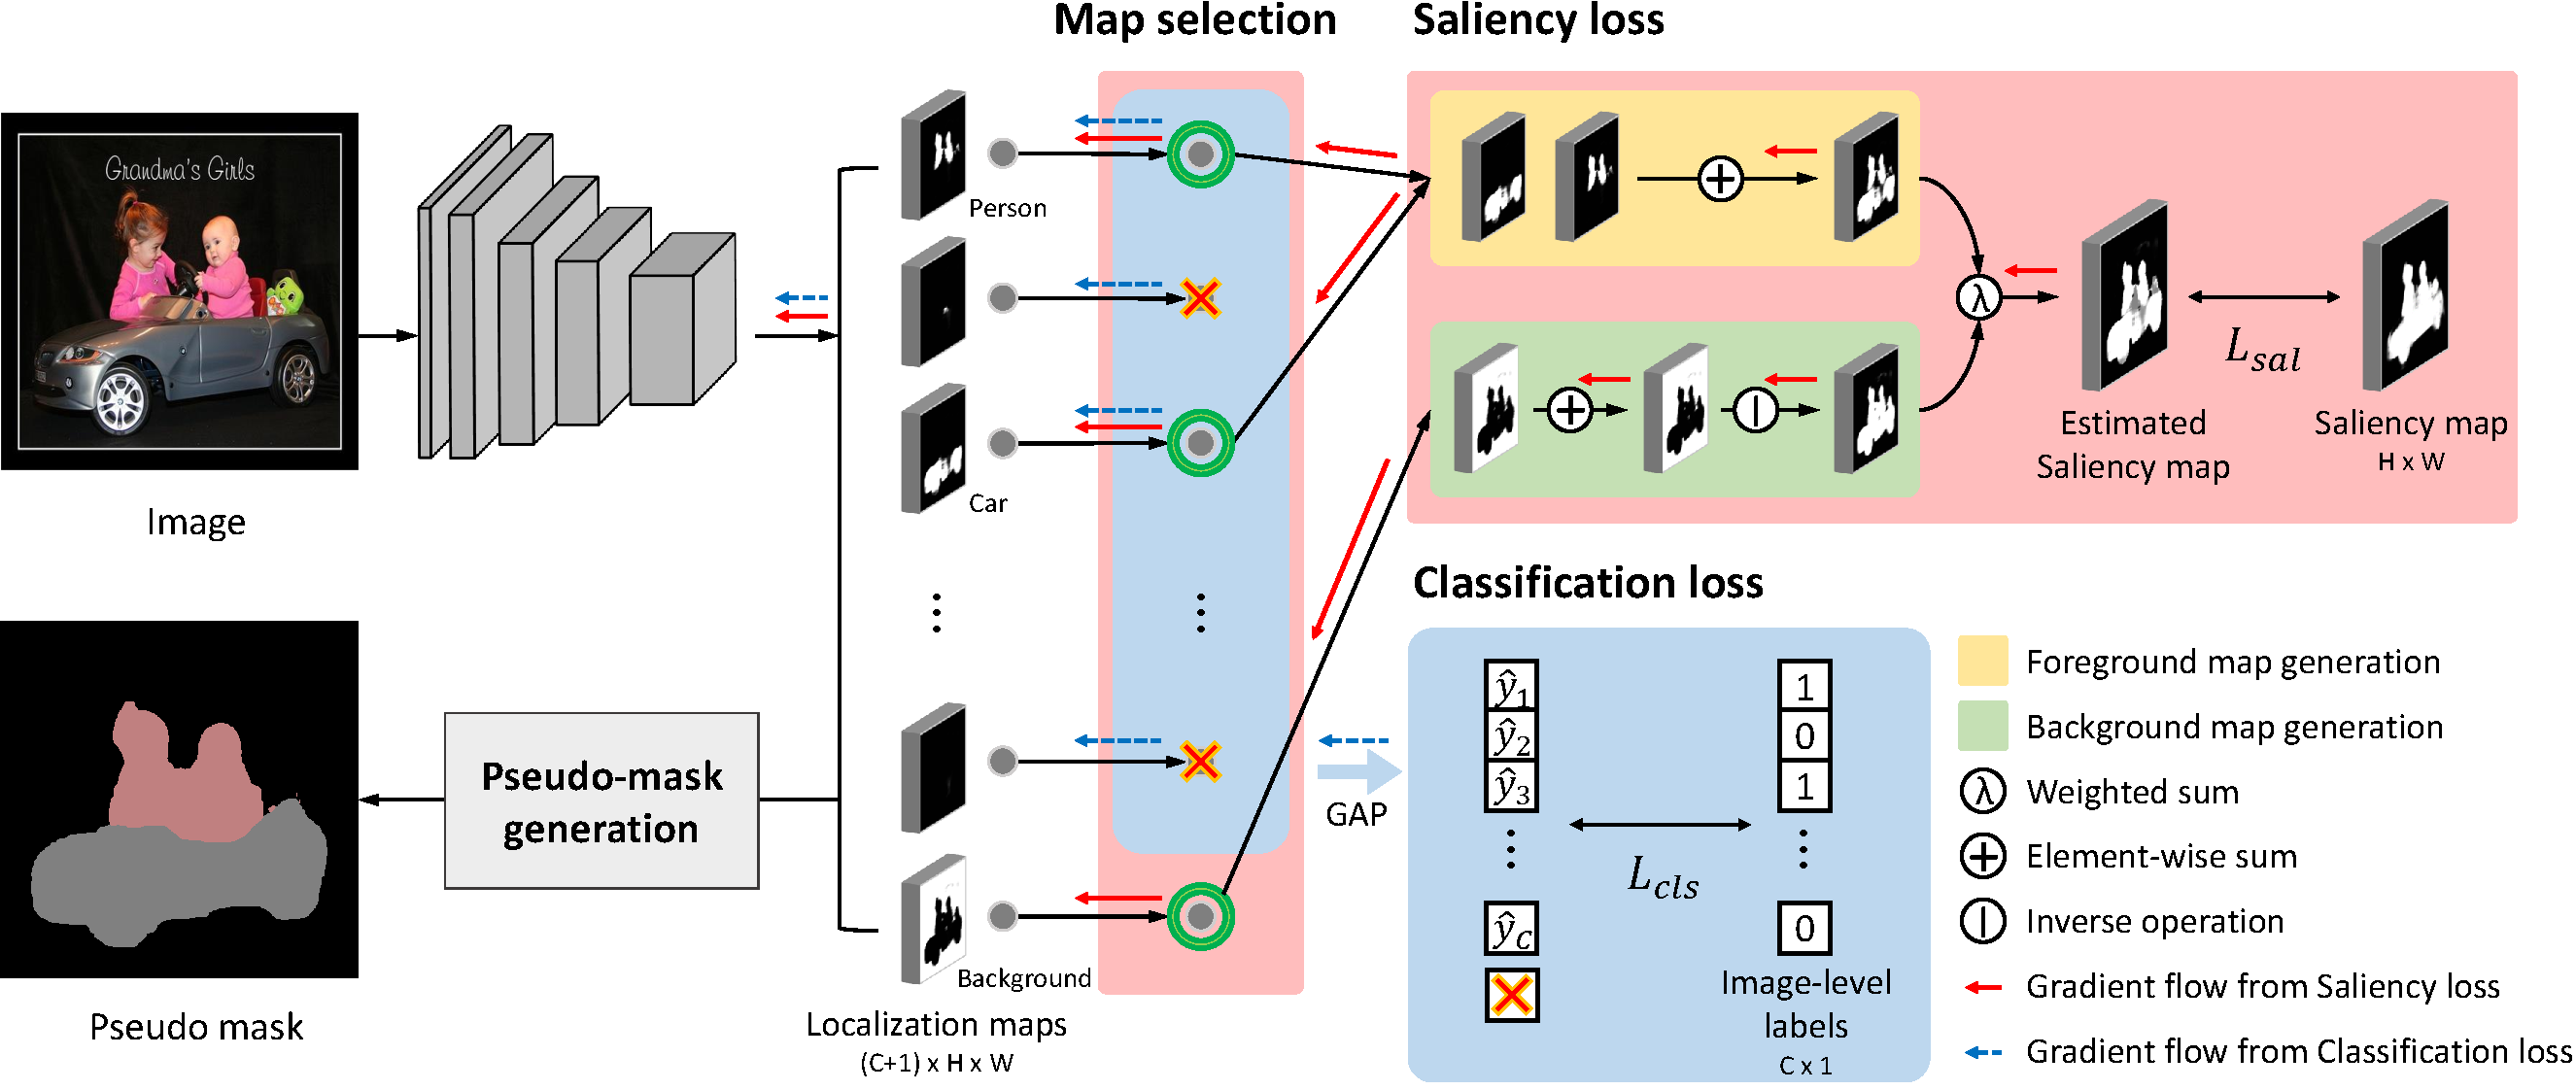
\includegraphics[width=16cm]{figures/framework.pdf}
\caption{우리의 EPS의 전체 프레임워크. $C+1$ 개의 지역화 맵이 백본 네트워크에서 생성됩니다. 실제 주목도 맵은 기성품 주목도 탐지 모델에서 생성됩니다. 대상 레이블에 대한 일부 지역화 맵은 선택적으로 사용되어 추정된 주목도 맵을 생성합니다 (Section~\ref{section3.2}). 전체 프레임워크는 주목도 손실과 분류 손실과 함께 공동으로 학습됩니다 (Section~\ref{section3.3}). } \vspace{-2mm}
\label{fig:framework}
\end{figure*}
